\DocumentMetadata{}
\documentclass[dvipsnames,12pt]{exam}
% compiles with
% latexmk -pdflatex=lualatex -pdf new.tex

\usepackage[top = 2cm, bottom = 3cm, left=1.5cm, right=1.5cm]{geometry}
\usepackage{microtype}
\usepackage{fontspec}
\usepackage{amssymb}
\usepackage{titlesec}
\usepackage{multicol}
\usepackage[shortlabels]{enumitem}
\usepackage{braket}
\usepackage{graphicx}
\usepackage{tikz}
\usepackage{pgfplots}
\usepgfplotslibrary{fillbetween}
\usetikzlibrary{intersections}
\graphicspath{{./img/}}
\usepackage{xcolor}
\usepackage{cancel}
\newcommand\Ccancel[2][black]{\renewcommand\CancelColor{\color{#1}}\cancel{#2}}
\usepackage{amsmath}
\usepackage{hyperref}
\usepackage{eso-pic}
\runningfooter{}{}{\thepage}
\runningheader{}{}{\scriptsize Aayush Bajaj | z5362216}

\hypersetup{
     colorlinks   = true,
     linkcolor    = RedViolet,
     citecolor    = gray
}

\titleformat{\section}{\normalfont\Large\bfseries}{{\color{RedViolet}\S}}{0.5em}{}
\titleformat{\subsection}{\normalfont\large\bfseries}{{\large \color{RedViolet}\S\S}}{0.5em}{}
\titleformat{\subsubsection}{\normalfont\bfseries}{{\color{RedViolet}\S\S\S}}{0.5em}{}

\parindent 0pt
%%% defs courtesy of Denis:
\newcommand{\N}{{\mathbb{N}}}
\newcommand{\C}{{\mathbb{C}}}
\newcommand{\D}{{\mathbb{D}}}
\newcommand{\F}{{\mathcal{F}}}
\renewcommand{\P}{{\mathcal{P}}} %careful with this, it redefines the usual P!
\newcommand{\R}{{\mathbb{R}}}
\newcommand{\Q}{{\mathbb{Q}}}
\newcommand{\T}{{\mathbb{T}}}
\newcommand{\Z}{{\mathbb{Z}}}
\newcommand{\ds}{\displaystyle}
\newcommand{\st}{\,:\,}
\renewcommand{\a}{{\mathbf a}}
\newcommand{\x}{{\mathbf x}}
\newcommand{\y}{{\mathbf y}}
\newcommand{\norm}[1]{\Vert #1 \Vert}
\renewcommand{\mod}[1]{\vert #1 \vert}
\newcommand\vecx{\boldsymbol{x}}
\newcommand\vecy{\boldsymbol{y}}
\newcommand{\zero}{\boldsymbol{0}}
\newcommand{\Arg}{\mathop{\mathrm{Arg}}}
\newcommand{\cl}{\mathop{\mathrm{cl}}}
\renewcommand{\Re}{\mathop{\mathrm{Re}}}
%%% end defs

%% theorems
\usepackage{amsthm}
\newtheorem{theorem}{Theorem}[section]
\newtheorem{corollary}{Corollary}[theorem]
\newtheorem{lemma}[theorem]{Lemma}
\newtheorem{prop}{Proposition}
\newtheorem*{notation}{Notation}
\newtheorem{remark}{Remark}
\newtheorem{claim}{Claim}

\theoremstyle{definition}
\newtheorem{definition}{Definition}[section]
%%%%%

\AddToShipoutPictureBG*{%  % Note the asterisk (*) - this is important!
  \AtPageCenter{%
    \makebox(0,0){%
      \rotatebox{45}{\textcolor{gray!30}{\fontsize{200}{100}\selectfont FINAL}}%
    }%
  }%
}

\author{Aayush Bajaj | z5362216}
\date{\today}
\title{MATH3611 | Assignment 3}

\begin{document}

\maketitle
\dotfill
\tableofcontents
\vspace{1cm}
\begin{center}
\includegraphics[width=0.2\textwidth]{logo.png}
\end{center}
\vspace{1cm}
\hrule

\newpage

%%%%%%%%%%%%%%%%%%%%%%%%%%%%%%%%%%%%%%%%%%%%%%%%%%%%%%%%%%%%%%%%%%%%%%%%%%%%%%%%
% Question 1
%%%%%%%%%%%%%%%%%%%%%%%%%%%%%%%%%%%%%%%%%%%%%%%%%%%%%%%%%%%%%%%%%%%%%%%%%%%%%%%%
\section{Question 1} \label{question1}

\begin{lemma}
For $x,y\in\R^{3}$ define
\[
d_{1}(x,y)=\sum_{i=1}^{3}\lvert x_{i}-y_{i}\rvert,
\qquad
d_{\infty}(x,y)=\max_{1\le i\le 3}\lvert x_{i}-y_{i}\rvert.
\]
Then
\[
d_{\infty}(x,y)\;\le\;d_{1}(x,y)\;\le\;3\,d_{\infty}(x,y).
\]
\end{lemma}

\begin{proof}
\emph{Lower bound.}
The maximum of non‑negative numbers is never larger than their sum, so  
$d_{\infty}(x,y)\le d_{1}(x,y)$.

\emph{Upper bound.}
Since each term $\lvert x_{i}-y_{i}\rvert\le d_{\infty}(x,y)$, summing over
$i=1,2,3$ yields $d_{1}(x,y)\le 3\,d_{\infty}(x,y)$.
\end{proof}

\begin{theorem}\label{thm:topology}
The metrics $d_{1}$ and $d_{\infty}$ induce the same topology on $\R^{3}$.
\end{theorem}

\begin{proof}
Fix $x\in\R^{3}$ and $\varepsilon>0$.

\smallskip
\textbf{$d_{1}$‑open $\implies$ $d_{\infty}$‑open.}
If $y\in B_{1}(x,\varepsilon)$, then
$d_{\infty}(x,y)\le d_{1}(x,y)<\varepsilon$; hence
\[
B_{1}(x,\varepsilon)\subset B_{\infty}(x,\varepsilon).
\]
Thus every $d_{1}$‑open set is $d_{\infty}$‑open.

\smallskip
\textbf{Converse $(\impliedby)$.}
Let $y\in B_{\infty}(x,\varepsilon)$.  
By the lemma, $d_{1}(x,y)\le 3\,d_{\infty}(x,y)<3\varepsilon$, so
\[
B_{\infty}(x,\varepsilon)\subset B_{1}(x,3\varepsilon).
\]
Hence every $d_{\infty}$‑open set is $d_{1}$‑open.

\smallskip
Because each topology is contained in the other, they coincide.
\end{proof}

\newpage

%%%%%%%%%%%%%%%%%%%%%%%%%%%%%%%%%%%%%%%%%%%%%%%%%%%%%%%%%%%%%%%%%%%%%%%%%%%%%%%%
% Question 2
%%%%%%%%%%%%%%%%%%%%%%%%%%%%%%%%%%%%%%%%%%%%%%%%%%%%%%%%%%%%%%%%%%%%%%%%%%%%%%%%
\section{Question 2} \label{question2}
\begin{definition}
    \[\tau = \set{\varnothing} \cup \set{U\subset \R:\R \setminus U \text{ is countable}}\]
\end{definition}

\begin{theorem}[A sequence $(x_n)_{n\in\N}\subset\R$ converges in $(\R,\tau)$ iff it is eventually constant]\label{thm2}
    \[\exists K\in \N: \forall n \ge K: x_n = x \iff x_n \xrightarrow{\tau} x\]

\end{theorem}
\begin{proof}
    $(\implies)$ Assume $x_n \xrightarrow{\tau}x$. Set \[C := \set{x_n:x_n\neq x}\] to be the countable collection of terms different from $x$, and set \[U:=\R \setminus C \cup \set{x}\] to be the neighbourhood.\\


    Since $\R\setminus U = C$ is countable, $U\in\tau$ and $x\in U$.\\


    By convergence, there exists $K$ such that $x_n\in U$ for all $n\ge K$. But if any $n\ge K$ with $x_n \neq x$, then $x_n \in C = \R\setminus U$ which contradicts $x_n\in U$. Hence $x_n=x \;\forall n \ge K$.\\



    $(\impliedby)$ Conversely, suppose $x_n=x$ for all $n\ge K$. Let $U\in \tau$ be any neighbourhood of $x$. Then $x_n \in U$ whenever $n\ge K$, so $x_n\xrightarrow{\tau} x$.

\end{proof}

\begin{corollary}
    For the sequence \[x_n=\begin{cases}1,& n\text{ odd},\\1-\dfrac1n, & n\text{ even}\end{cases}\] no tail is constant, hence \[x_n \not\xrightarrow{\tau}x\quad\text{for any }x\in\R\]
\end{corollary}
\begin{proof}
    The set of odd indices is infinite so $x_{2k-1} = 1$ occurs infinitely often. Likewise, the even subsequence $(1-\tfrac1{2k})_{k\ge1}$ takes infinitely many distinct values. Thus the sequence $(x_n)_{n\in\N}$ cannot be eventually constant and by \ref{thm2} does not converge in the co-countable topology.
\end{proof}

\newpage

%%%%%%%%%%%%%%%%%%%%%%%%%%%%%%%%%%%%%%%%%%%%%%%%%%%%%%%%%%%%%%%%%%%%%%%%%%%%%%%%
% Question 3
%%%%%%%%%%%%%%%%%%%%%%%%%%%%%%%%%%%%%%%%%%%%%%%%%%%%%%%%%%%%%%%%%%%%%%%%%%%%%%%%
\section{Question 3}

\begin{theorem}[Uniform convergence on closed sub‑intervals]\label{thm:innerUniform}
  Let \[ S(x)=\sum_{n=0}^{\infty} a_n x^{n}, \qquad x\in\R, \] be a power series with (finite) radius of convergence \(R>0\). Then for every \(\varepsilon>0\) the series \(S\) converges \emph{uniformly} on the closed interval \[ [-\,R+\varepsilon,\; R-\varepsilon]. \]
\end{theorem}
\begin{proof}
  Fix $\varepsilon>0$ and set $r:=R-\varepsilon>0$.  Let $I=[-\,r,r]$.\\

  For $n\in\mathbb N$ define $f_n(x):=a_n x^n$ on $I$.\\

  Because $|x|\le r$ for all $x\in I$, \[ |f_n(x)|\le |a_n|\,r^{\,n}=:\,M_n \quad (x\in I).
  \]

  Since $|r|<R$, the power series converges \emph{absolutely} at $x^\ast=r$; hence the series \(\sum_{n=0}^{\infty}M_n=\sum_{n=0}^{\infty}|a_n|r^{\,n}\) converges.\\

  With $|f_n(x)|\le M_n$ for every $x\in I$, the Weierstrass $M$‑test guarantees that \(\sum_{n=0}^{\infty}f_n(x)\) converges uniformly on $I$, i.e. \[ \sum_{n=0}^{\infty}a_n x^n \text{ converges uniformly on } [-R+\varepsilon,R-\varepsilon]. \]
\end{proof}

\newpage

%%%%%%%%%%%%%%%%%%%%%%%%%%%%%%%%%%%%%%%%%%%%%%%%%%%%%%%%%%%%%%%%%%%%%%%%%%%%%%%%
% Question 4
%%%%%%%%%%%%%%%%%%%%%%%%%%%%%%%%%%%%%%%%%%%%%%%%%%%%%%%%%%%%%%%%%%%%%%%%%%%%%%%%
\section{Question 4}

For each integer $k\ge1$ define
\[ f_k : [0,1] \longrightarrow \R, \qquad f_k(x)=\max\{0,1-4k^{2}|\,x-\tfrac{1}{k^{2}}|\}.\]

\begin{enumerate}[a)]
%------------------------------------------------------------------------------%
\item \textbf{Sketches of $f_1,f_2,f_3$.}

\begin{figure}[h]
\centering
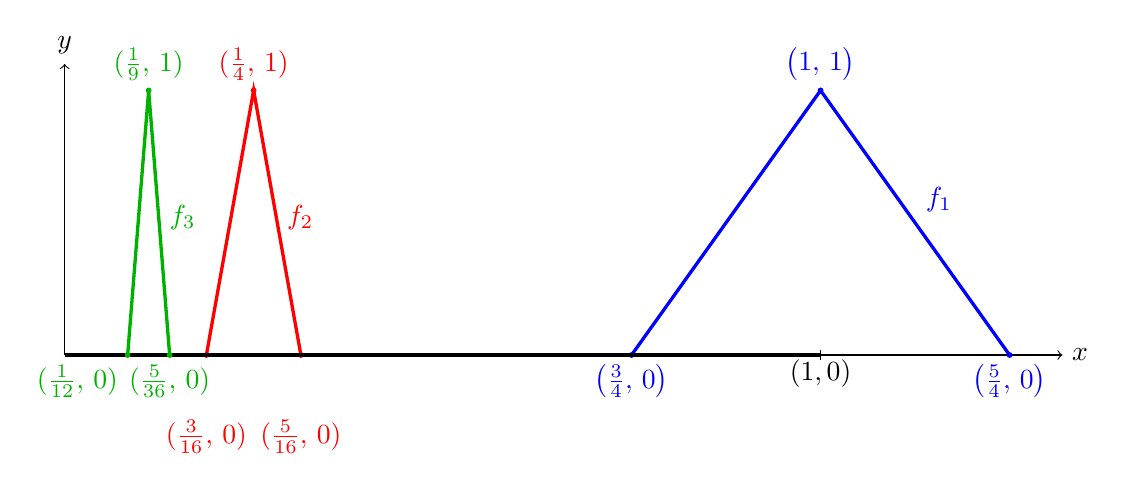
\begin{tikzpicture}[x=8cm,y=2.8cm,scale=1.2]
  % axes -----------------------------------------------------------------------
  \draw[->] (0,0) -- (1.32,0) node[right] {$x$};
  \draw[->] (0,0) -- (0,1.10) node[above] {$y$};

  %----------------------------------------------------------------------------%
  %  f1  (k = 1)  -------------------------------------------------------------%
  %  support = [3/4 , 5/4],   apex at (1 , 1)
  \draw[very thick,blue]
        (3/4,0) -- (1,1) -- (5/4,0)
        node[midway,above right,blue] {$f_{1}$};

  \filldraw[blue] (3/4,0) circle (0.7pt)
        node[below] {$\bigl(\tfrac34,\,0\bigr)$};
  \filldraw[blue] (1,1)   circle (0.7pt)
        node[above] {$\bigl(1,\,1\bigr)$};
  \filldraw[blue] (5/4,0) circle (0.7pt)
        node[below] {$\bigl(\tfrac54,\,0\bigr)$};

  %----------------------------------------------------------------------------%
  %  f2  (k = 2)  -------------------------------------------------------------%
  %  support = [3/16 , 5/16],   apex at (1/4 , 1)
  \draw[very thick,red]
        (3/16,0) -- (1/4,1) -- (5/16,0)
        node[midway,right,pos=0.48,red] {$f_{2}$};

  \filldraw[red] (3/16,0) circle (0.7pt)
        node[below=20pt] {$\tiny(\tfrac{3}{16},\,0)$};
  \filldraw[red] (1/4,1)  circle (0.7pt)
        node[above] {$\tiny(\tfrac14,\,1)$};
  \filldraw[red] (5/16,0) circle (0.7pt)
        node[below=20pt] {$\tiny(\tfrac{5}{16},\,0)$};

  %----------------------------------------------------------------------------%
  %  f3  (k = 3)  -------------------------------------------------------------%
  %  support = [1/12 , 5/36],   apex at (1/9 , 1)
  \draw[very thick,green!70!black]
        (1/12,0) -- (1/9,1) -- (5/36,0)
        node[midway,right,pos=.48,green!70!black] {$f_{3}$};

  \draw[very thick,black] (0,0) -- (1,0);
  \draw (1,-0.02) -- (1,0.02) node[below] {$(1,0)$};
  \filldraw[green!70!black] (1/12,0) circle (0.7pt)
        node[below left] {$\tiny(\tfrac1{12},\,0)$};
  \filldraw[green!70!black] (1/9,1)  circle (0.7pt)
        node[above] {$\tiny(\tfrac19,\,1)$};
  \filldraw[green!70!black] (5/36,0) circle (0.7pt)
        node[below] {$\tiny(\tfrac5{36},\,0)$};
\end{tikzpicture}
\end{figure}

%------------------------------------------------------------------------------%
\item \textbf{Support of $f_k$.}

Solve
\( 1-4k^{2}\lvert x-\tfrac1{k^{2}}\rvert>0 \iff \lvert x-\tfrac1{k^{2}}\rvert<\tfrac1{4k^{2}} \).
Hence
\[ \boxed{ \operatorname{supp}(f_k) =\left(\tfrac{3}{4k^{2}},\,\tfrac{5}{4k^{2}}\right) \cap[0,1], k\ge1} \]
whereby,
\[
  \operatorname{supp}(f_1)=(\tfrac34,\,1],\qquad
  \operatorname{supp}(f_k)=\bigl(\tfrac{3}{4k^{2}},\,\tfrac{5}{4k^{2}}\bigr)
  \ (k\ge2).
\]

%------------------------------------------------------------------------------%
\item \textbf{Pointwise convergence and failure of uniform convergence of}
      \[ S(x):=\sum_{k=1}^{\infty}\frac{f_k(x)}{k}, \qquad x\in[0,1]. \]

\begin{enumerate}[label=(\roman*)]
%..............................................................................%
\item \emph{Pointwise convergence.}

Fix $x\in(0,1]$.  
The inequality
\( \frac{3}{4k^{2}}<x<\frac{5}{4k^{2}} \)
is equivalent to
\[ A(x):=\sqrt{\tfrac{3}{4x}} <k< B(x):=\sqrt{\tfrac{5}{4x}}. \]
Whose length is \[ L(x):=B(x)-A(x) =\frac{\sqrt5-\sqrt3}{2\sqrt{x}} <\frac{0.253}{\sqrt{x}}<\infty, \]
so the interval holds at most
\( \left\lceil L(x)\right\rceil \)
integers.  Hence only finitely many \(k\) satisfy \(f_k(x)\neq0\); the
series \(S(x)\) reduces to a finite sum and converges.
For \(x=0\) every term is \(0\), so \(S(0)=0\).  
Thus \(S\) converges for every \(x\in[0,1]\).

%..............................................................................%
\item \emph{Failure of uniform convergence.}

Let \(S_N(x):=\sum_{k=1}^{N}\frac{f_k(x)}{k}\).
For \(N\ge10\) choose 
\[ x_N:=\frac1{N^{2}}\in[0,1]. \]

\medskip
\begin{claim}
For every
\( k\in\left[N+1,N+\lfloor N/10\rfloor\right] \)
we have
\( f_k(x_N)\ge\frac12. \)
\end{claim}


\begin{proof}
For such \(k\),
\[ \left|x_N-\tfrac1{k^{2}}\right| =\frac{|k^{2}-N^{2}|}{k^{2}N^{2}} =\frac{(k-N)(k+N)}{k^{2}N^{2}} \le\frac{(N/10)(11N/10)}{k^{2}N^{2}} <\frac{11}{100\,k^{2}} <\frac1{8\,k^{2}} <\frac1{4k^{2}},
\]
so \(x_N\in\operatorname{supp}(f_k)\) and \(f_k(x_N)=1-4k^{2}\lvert x_N-\tfrac1{k^{2}}\rvert\ge\frac12\). 
\end{proof}

\medskip
Therefore the tail \(T_N(x):=\sum_{k>N}\frac{f_k(x)}{k}\) satisfies
\[ T_N(x_N) \ge \frac12 \sum_{k=N+1}^{N+\lfloor N/10\rfloor}\frac1k \ge \frac12\ln\left(1+\tfrac1{10}\right) =:c>0 \qquad(N\ge10), \]
using $\sum_{k=m}^n \tfrac1k \ge \ln\dfrac{n}{m}, \forall n,m\in\N,n\ge m\ge 1$:
\[ \|S-S_N\|_{\infty} =\sup_{x\in[0,1]}|S(x)-S_N(x)| \ge |T_N(x_N)| \ge c \quad\text{for all }N\ge10, \]
so \(\|S-S_N\|_{\infty}\not\to0\).  
The convergence of the series is therefore \emph{not} uniform on \([0,1]\).
\end{enumerate}
\end{enumerate}
\end{document}
